\documentclass{beamer}
\usepackage[utf8]{inputenc}

\usetheme{Madrid}
\usecolortheme{default}
\usepackage{amsmath,amssymb,amsfonts,amsthm}
\usepackage{txfonts}
\usepackage{tkz-euclide}
\usepackage{listings}
\usepackage{adjustbox}
\usepackage{array}
\usepackage{tabularx}
\usepackage{gvv}
\usepackage{lmodern}
\usepackage{circuitikz}
\usepackage{tikz}
\usepackage{graphicx}

\setbeamertemplate{page number in head/foot}[totalframenumber]

\usepackage{tcolorbox}
\tcbuselibrary{minted,breakable,xparse,skins}



\definecolor{bg}{gray}{0.95}
\DeclareTCBListing{mintedbox}{O{}m!O{}}{%
  breakable=true,
  listing engine=minted,
  listing only,
  minted language=#2,
  minted style=default,
  minted options={%
    linenos,
    gobble=0,
    breaklines=true,
    breakafter=,,
    fontsize=\small,
    numbersep=8pt,
    #1},
  boxsep=0pt,
  left skip=0pt,
  right skip=0pt,
  left=25pt,
  right=0pt,
  top=3pt,
  bottom=3pt,
  arc=5pt,
  leftrule=0pt,
  rightrule=0pt,
  bottomrule=2pt,
  toprule=2pt,
  colback=bg,
  colframe=orange!70,
  enhanced,
  overlay={%
    \begin{tcbclipinterior}
    \fill[orange!20!white] (frame.south west) rectangle ([xshift=20pt]frame.north west);
    \end{tcbclipinterior}},
  #3,
}
\lstset{
    language=C,
    basicstyle=\ttfamily\small,
    keywordstyle=\color{blue},
    stringstyle=\color{orange},
    commentstyle=\color{green!60!black},
    numbers=left,
    numberstyle=\tiny\color{gray},
    breaklines=true,
    showstringspaces=false,
}
\begin{document}

\title 
{2.10.63}
\date{September 12,2025}


\author 
{Kishora Karthik-EE25BTECH11034}
\frame{\titlepage}
\begin{frame}{Question}
A vector $\vec{A}$ has components $A_1, A_2, A_3$ in a right-handed rectangular Cartesian coordinate system $oxyz$. The coordinate system is rotated about the $x$-axis through an angle $\frac{\pi}{2}$. Find the components of $\vec{A}$ in the new coordinate system in terms of $A_1, A_2, A_3$.\\
\end{frame}



\begin{frame}{ Solution}
In the original coordinate system $S$,
\begin{align}
    \vec{A_S} = \myvec{ A_1 \\ A_2 \\ A_3}  
\end{align}
Let the new coordinate system be $S'$, obtained by rotating $S$ about the $x$-axis by an angle $\theta = \frac{\pi}{2}$. The components of the same vector $\vec{A}$ in the new system are,
\begin{align}
    \myvec{A'_1 \\ A'_2 \\ A'_3}   = R \myvec{A_1 \\ A_2 \\ A_3} 
\end{align}
where $R$ is the rotation matrix.
\end{frame}

\begin{frame}{Solution}
For a rotation of the coordinate system by an angle $\theta$ about the $x$-axis, 
\begin{align}
    R_x(\theta) = \myvec{1 & 0 & 0 \\ 0 & \cos\theta & \sin\theta \\ 0 & -\sin\theta & \cos\theta}  
\end{align}
Given, $\theta = \frac{\pi}{2}$.So,
\begin{align}    
R = \myvec{ 1 & 0 & 0 \\ 0 & \cos(\frac{\pi}{2}) & \sin(\frac{\pi}{2}) \\ 0 & -\sin(\frac{\pi}{2}) & \cos(\frac{\pi}{2})}   = \myvec{ 1 & 0 & 0 \\ 0 & 0 & 1 \\ 0 & -1 & 0}  
\end{align}
\end{frame}
\begin{frame}{Solution}
\begin{align}
    \myvec{A'_1 \\ A'_2 \\ A'_3}  = \myvec{1 & 0 & 0 \\ 0 & 0 & 1 \\ 0 & -1 & 0}   \myvec{ A_1 \\ A_2 \\ A_3}  
\end{align}
\begin{align}
A'_1 &= (1 \cdot A_1) + (0 \cdot A_2) + (0 \cdot A_3) = A_1 \\
A'_2 &= (0 \cdot A_1) + (0 \cdot A_2) + (1 \cdot A_3) = A_3 \\
A'_3 &= (0 \cdot A_1) + (-1 \cdot A_2) + (0 \cdot A_3) = -A_2
\end{align}
\begin{align}
\implies \myvec{A'_1 \\ A'_2 \\ A'_3} =\myvec{ A_1 \\ A_3 \\ -A_2} 
\end{align}
$\therefore$ The components of the vector $\vec{A}$ in the new coordinate system are:
$A'_1 = A_1$, $A'_2 = A_3$ and $A'_3 = -A_2$.
\end{frame}
\begin{frame}{Plot}
    \centering
    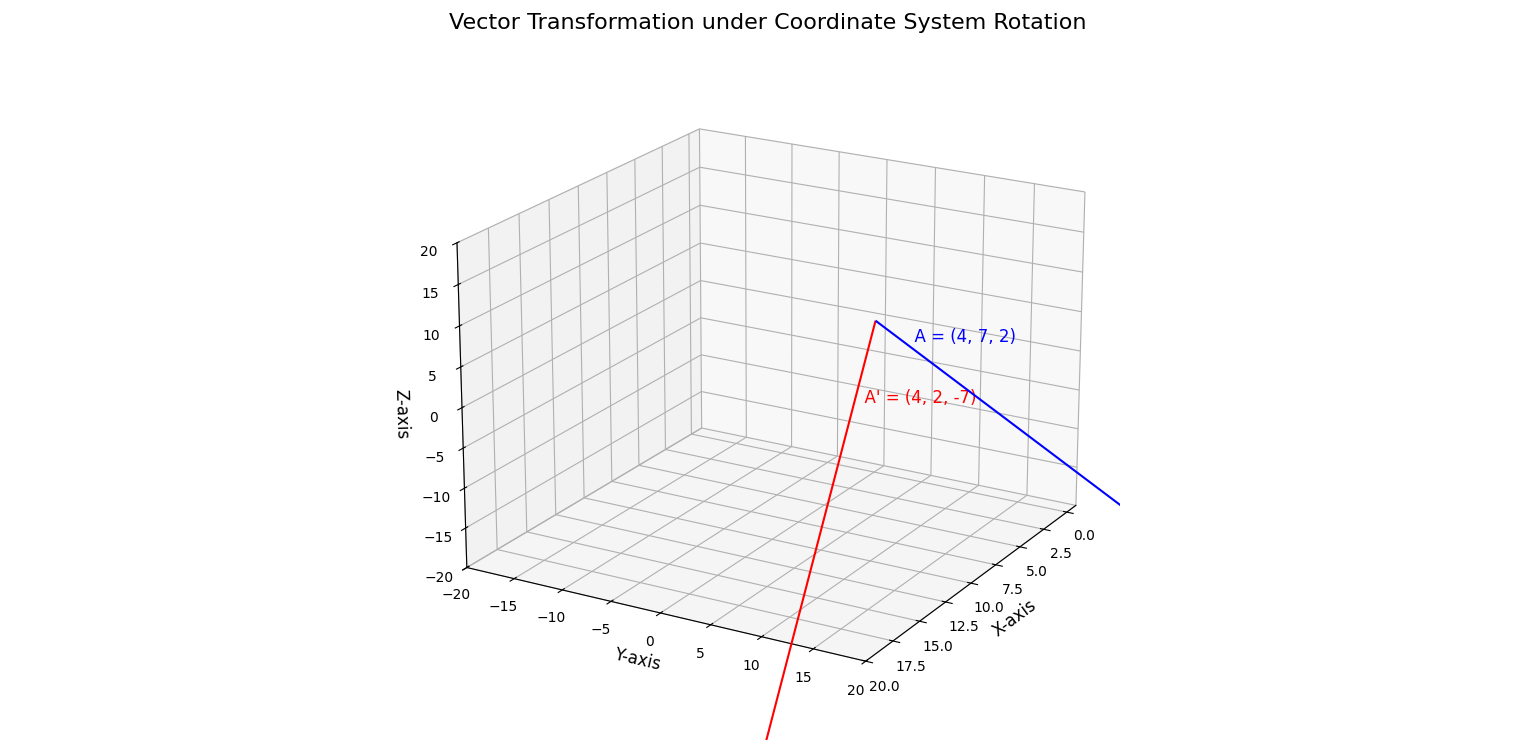
\includegraphics[width=\columnwidth, height=1\textheight, keepaspectratio]{figs/fig1.png} 
\end{frame}

\end{document}


